\section{Experiments}
\label{sec:exp}
In this section, we conduct extensive experiments for \gencliqjoin on both unlabelled and labelled data graphs. Here, we only consider undirected graph matching because an undirected edge can be regarded as two directed edges. We will show the experimental results over the optimizations we have done to \cliquejoin.
\subsection{Experimental Settings}
\stitle{Environments.} We use a cluster of 10 nodes connected via a 10Gpbs switch, and each node has 64GB memory, 1TB disk and 1 Intel Xeon CPU E3-1220 V6 3.00GHz with 4 physical cores. We implement \cliquejoin in \timely dataflow system \footnote{\url{https://github.com/frankmcsherry/timely-dataflow}} using Rust 1.27. We use 10 machines and each machine uses 3 workers by default.

\stitle{Metrics.} We measure query time $T$ from the average time of three runs. The query time is actually the slowest worker's running time during each run, which excludes graph loading time as it is negligible compared to query time. We set batch size to 10,000 and threshold to 10,000,000 by default in $\code{BatchJoin}$.

\stitle{Preprocessing Datasets.} We preprocess each dataset as follows: we treat it as a simple undirected graph by removing self-loop and duplicate edges, and reorder the node id according to the degree and represent it using Compressed Sparse Raw (CSR)\footnote{\url{https://en.wikipedia.org/wiki/Sparse_matrix}}.

\subsection{Unlabelled Matching}
\label{sec:unlabelled_matching}
\stitle{Datasets.} We evaluate 3 real graphs of different sizes and types. The sources of these graphs are from Snap\footnote{\url{http://snap.stanford.edu/data/index.html}} and WebG\footnote{\url{http://law.di.unimi.it/datasets.php}}. We consider the following two graph types: Social Network (Soc) and Web Graph (Web).  We list the evaluated graphs in \reftable{unl_datasets}. Note that both $|V(G)|$ and $|E(G)|$ are in millions. 

\begin{table}
\centering
 \begin{tabular}{|c|c|c|c|c|c|c|} 
 \hline
 Datasets & Name & $|V(G)|/mil$ & $|E(G)|/mil$ & $\overline{d(G)}$ & $D(G)$ \Ts\Bs \\
 \hline\hline
 livejournal & LJ & 4.85 & 43.37 & 8.9 & 20,333  \\
  \hline
 orkut & OK & 3.07 & 117.19 & 38.1 & 33,313 \\
 \hline
uk2002 & UK & 18.5 & 298.11 & 16.1 & 194,955\\
\hline
 \end{tabular}
\caption{The Unlabelled Datasets.}
\label{tab:unl_datasets}
\end{table}

\stitle{Queries.} The five queries denoted by $q_1$ to $q_5$ are illustrated in \reffig{unlq}, where the number of nodes vary from 4 to 5 and the number of edges vary from 4 to 10. We assign the order of the nodes for symmetry breaking\cite{Grochow2007} under each query graph. Here, we have considered all queries for fair comparisons.

\begin{figure}[htb]
  \centering
  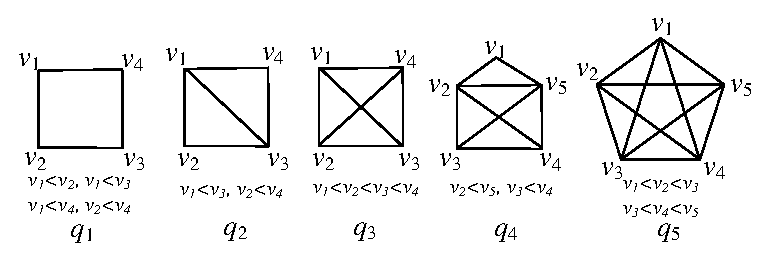
\includegraphics[scale=0.6]{figures/unlq.eps}
  \caption{\small{Unlabelled Queries.}}
  \label{fig:unlq}
\end{figure}

\stitle{Exp1 - Vary Queries.} We compare \gencliqjoin with \cliquejoin by testing all queries on LJ, which is shown in \reffig{vary_query}. Note that for better presentation, the ordinate is calculated by $logT$, where $T$ is the query time. We can see that for enumerating the join unit $q_3$(4-clique) and $q_5$(5-clique), \gencliqjoin outperforms \cliquejoin by more than one order of magnitude. For $q_2$, \gencliqjoin is 2 times faster than \cliquejoin. However, \cliquejoin outperforms \gencliqjoin in $q_1$ and $q_5$. TODO: Explain them.

\begin{figure}[htb]
  \centering
  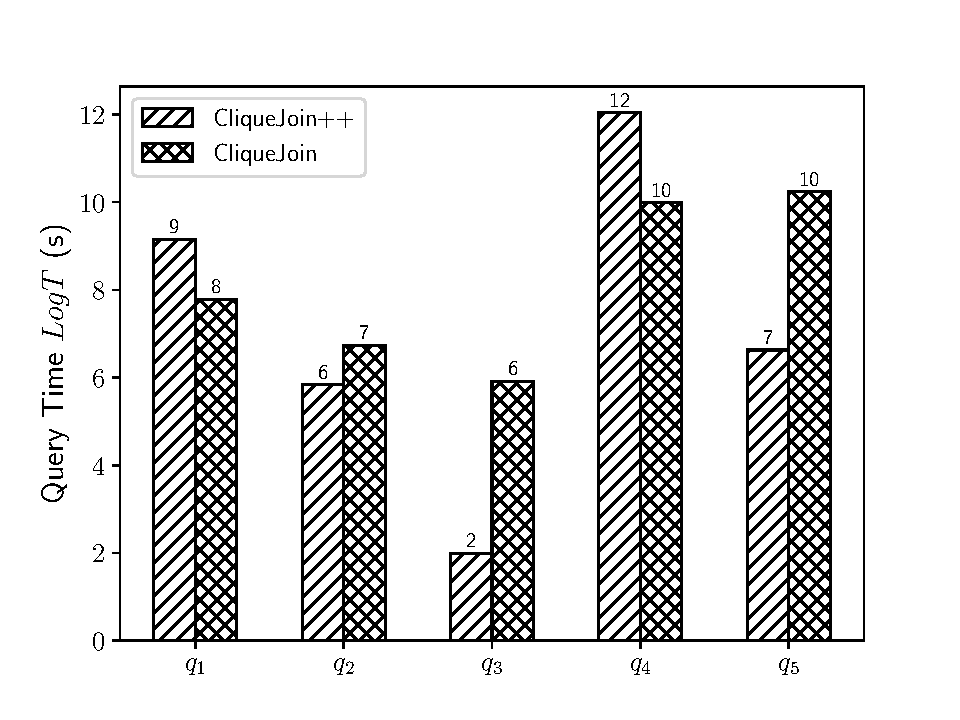
\includegraphics[scale=0.4]{figures/exp1.pdf}
  \caption{\small{Vary Queries.}}
  \label{fig:vary_query}
\end{figure}

\stitle{Exp2 - Vary Datasets.} We compare \gencliqjoin with \cliquejoin by querying $q_2$ and $q_5$ on all datasets in order to show the good performance over different data properties. The results are shown in \reffig{vary_dataset}. We can see that, when querying $q_2$, \gencliqjoin generally outperforms \cliquejoin by around 2 times. When querying $q_5$, \gencliqjoin is 3 to 10 times faster than \cliquejoin. 

\begin{figure}[htb]
  \flushleft
  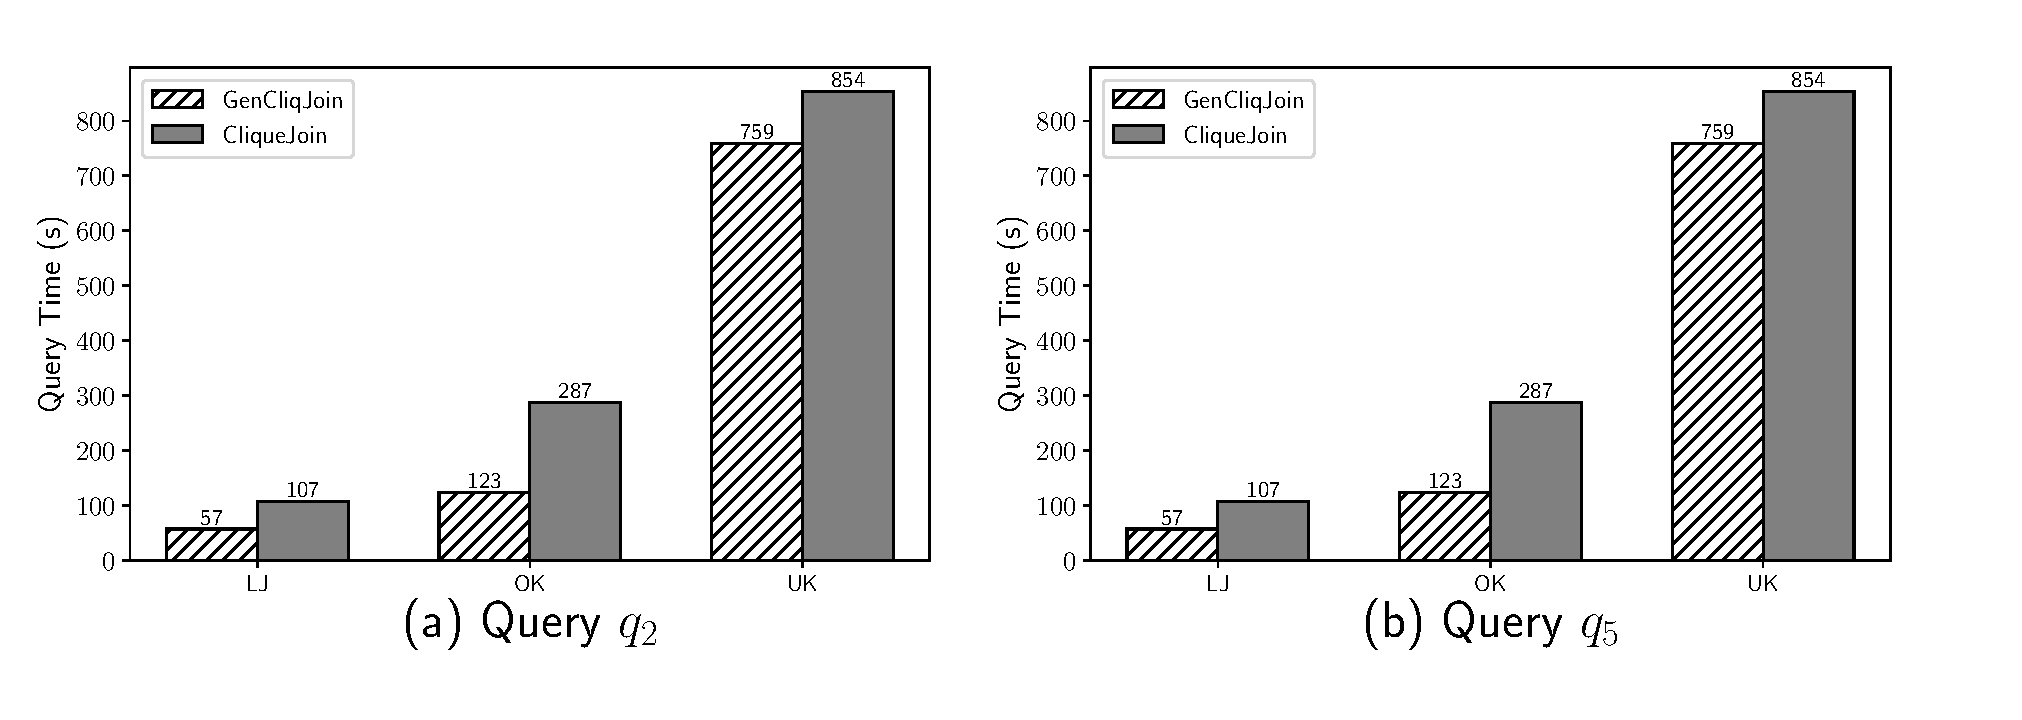
\includegraphics[scale=0.3]{figures/exp2.pdf}
  \caption{\small{Vary Datasets.}}
  \label{fig:vary_dataset}
\end{figure}


\stitle{Exp3 - Scalability.} We compare the scalability of \gencliqjoin with \cliquejoin on LJ using $q_2$ by varying number of nodes(6, 8, 10) used in the cluster, whose results are shown in \reffig{unl_sca}. We can see that \gencliqjoin is in general 2 times faster than \cliquejoin.

\begin{figure}[htb]
  \centering
  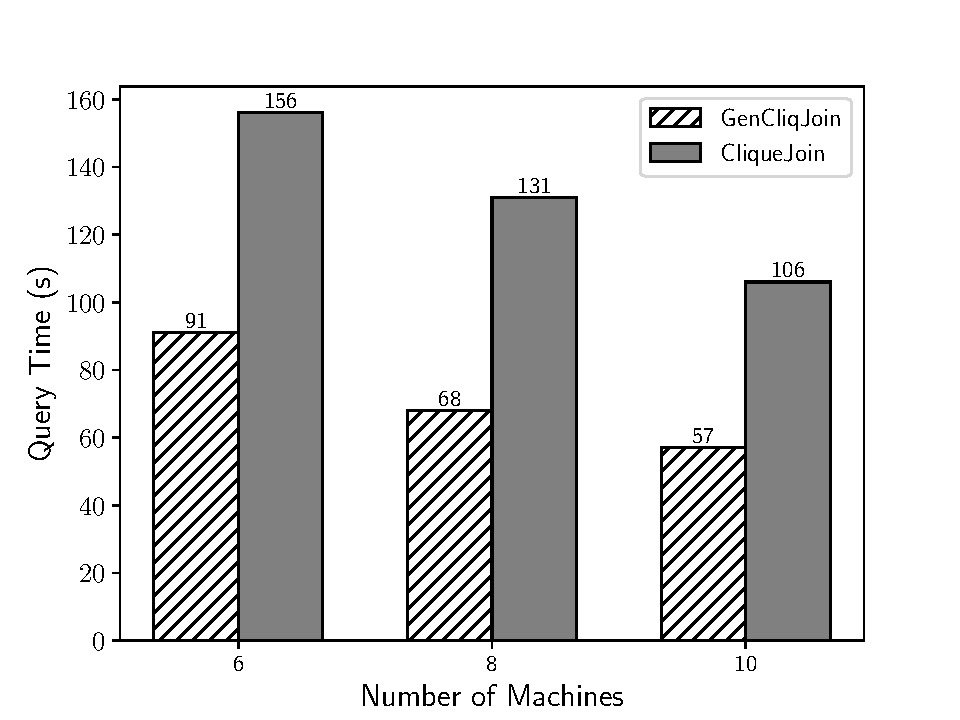
\includegraphics[scale=0.37]{figures/exp3.pdf}
  \caption{\small{Unlabelled Scalability.}}
  \label{fig:unl_sca}
\end{figure}


\subsection{Labelled Matching.} We use LDBC social network benchmarking (SNB)\cite{Ldbc} for labelled matching experiment for the lack of big public labelled graphs. SNB provides a data generator that can generate synthetic social networks of statistics, and a document\cite{LdbcDoc} that describes the benchmarking tasks, which are actually doing subgraph matching. To the best of our knowledge, there are few experiments of distributed labelled subgraph matching on large datasets. Therefore, in this section, we will just demonstrate the effectiveness and scalability of \gencliqjoin when doing labelled subgraph matching.

\stitle{Datasets.} We list the datasets and their statistics in \reftable{l_datasets}. All datasets are generated using the "Facebook" mode with a span of 3 years. The dataset's name, denoted as DG$x$, represents a scale factor of $x$. As mentioned before, we first parse the graph into undirected simple graph. Then we remove all properties except the node types as labels, and the label is encoded as an integer to accelerate the matching.

\begin{table}
\centering
 \begin{tabular}{|c|c|c|c|c|c|c|} 
 \hline
 Name & $|V(G)|/mil$ & $|E(G)|/mil$ & $\overline{d(G)}$  & $D(G)$ & \#Labels \Ts\Bs \\
 \hline\hline
 DG01 & 3.2 & 17.24 & 10.84 & 464,368  & 11 \\
  \hline
 DG03 & 9.28 & 52.65 & 11.3 & 1,346,287 & 11 \\
 \hline
 DG10 & 29.99 & 176.48 & 11.77 & 4,282,812 & 11 \\
\hline
 DG30 & 88.79 & 540.51 & 12.17 &  12,684,488 & 11 \\
\hline
 DG60 & 187.11 & 1246.66 & 13.32 & 26,639,563 & 11 \\
\hline
 \end{tabular}
\caption{The Labelled Datasets.}
\label{tab:l_datasets}
\end{table}

\stitle{Queries.} The labelled queries are shown in \reffig{lq}, which are generated from SNB's tasks with following rules: (1) removing the direction of edges and edge labels; (2) using one-hop edge for multi-hop edges; (3) removing the "no edge" and unconnected graph condition; (4) removing all properties except the node type as its label. For (1), we do the adaptation for simplicity although we can support that case. We adapt (2) and (3) for consistency with the subgraph matching problem studied in this paper. We adapt (4) for our implementation currently can not support property graphs.

\begin{figure}[htb]
  \centering
  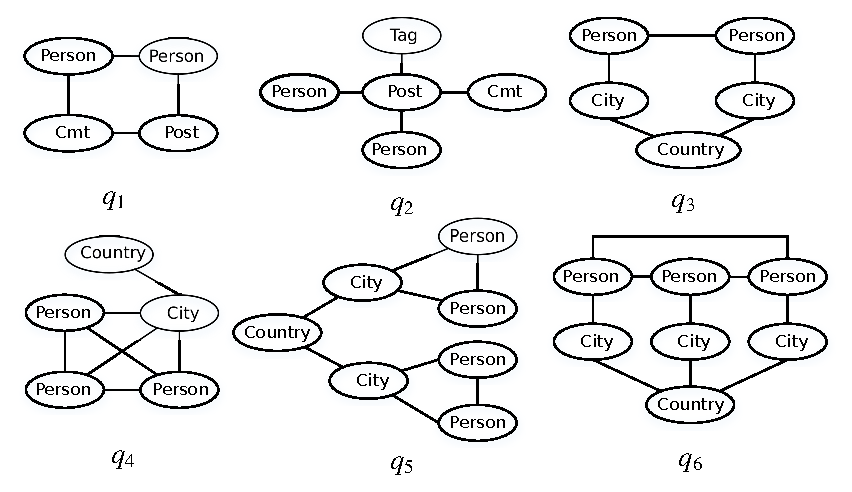
\includegraphics[scale=0.6]{figures/lq.eps}
  \caption{\small{Labelled Queries.}}
  \label{fig:lq}
\end{figure}

\stitle{Exp4 - All Labelled Queries.} We perform \gencliqjoin for all queries on all datasets, and the results are illustrated in \reffig{all_lq}(whose ordinate is the logarithm of query time $T$). We can see that \gencliqjoin can finish subgraph matching in tens of seconds for $q_2, q_3, q_4, q_5, q_6$ in all data graphs, even if DG60 is a billion scale graph. We notice that the query time for $q_1$ increases sharply when the dataset becomes larger. The reason is that the algorithm spends a lot of time computing the stars' matches in $q_1$($q_1$ is decomposed to two 2-star(s)) due to the poor filter information of $q_1$'s join units in data graph.

\begin{figure}[htb]
  \centering
  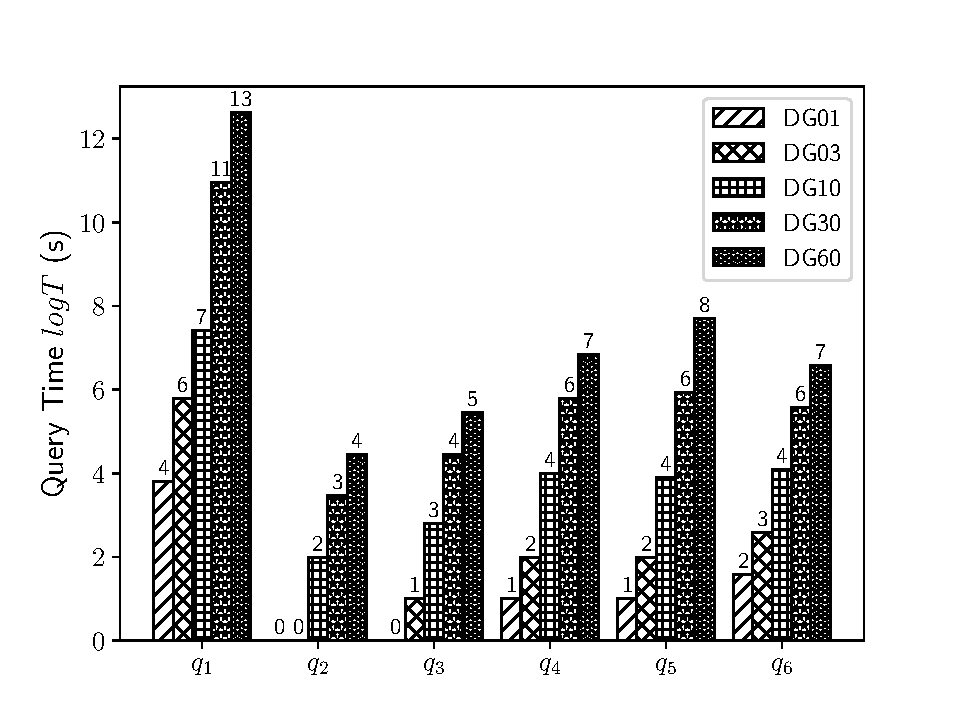
\includegraphics[scale=0.4]{figures/exp4.pdf}
  \caption{\small{All Labelled Queries.}}
  \label{fig:all_lq}
\end{figure}

\stitle{Exp5 - Labelled Scalability.} We evaluate the labelled matching scalability of $q_1$ and $q_4$ on DG10 by varying the number of nodes used in the cluster(6, 8, 10), and the results are demonstrated in \reffig{l_sca}. We can see that when decreasing the number of machines used in the cluster, the query time slightly increases, which shows that \gencliqjoin has great scalability for labelled matching.

\begin{figure}[htb]
  \centering
  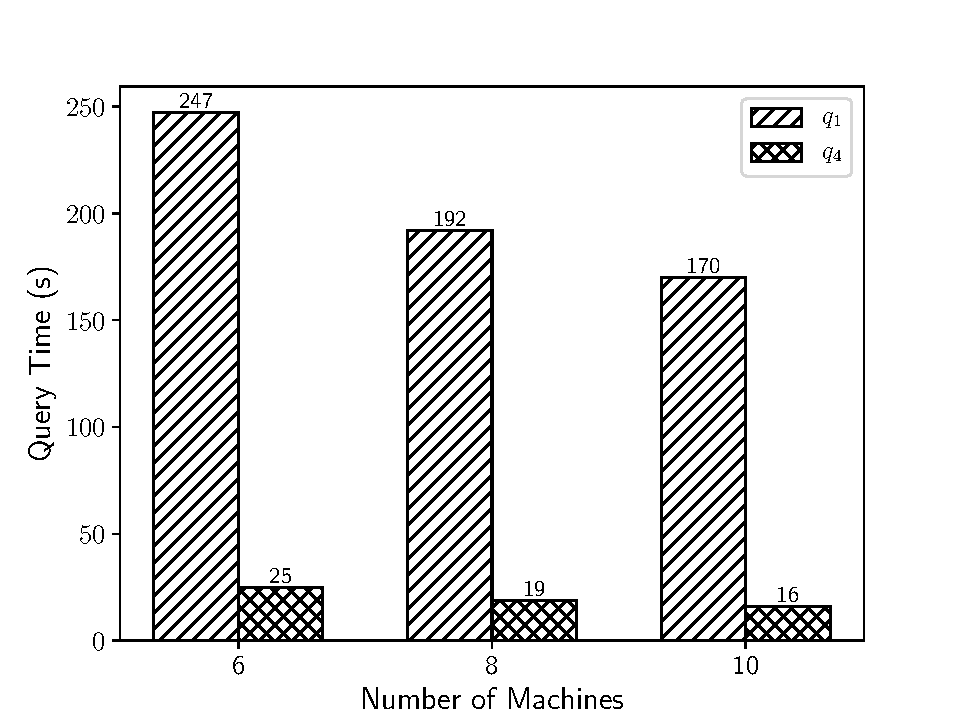
\includegraphics[scale=0.4]{figures/exp5.pdf}
  \caption{\small{Labelled Scalability.}}
  \label{fig:l_sca}
\end{figure}
